\documentclass[11.5pt]{sig-alternate} % sets document style to sig-alternate
% packages
% typesetting
%\usepackage{dirtytalk} % typset quotations easier (\say{stuff})
\usepackage{hanging} % hanging paragraphs
\usepackage[defaultlines=3,all]{nowidow} % avoid widows
\usepackage[pdfpagelabels=false]{hyperref} % produce hypertext links, includes backref and nameref
\usepackage{xurl} % defines url linebreaks, loads url package
\usepackage{microtype}
\usepackage{textgreek}
%\usepackage{textcomp}
%\newcommand{\texttildemid}{\raisebox{0.4ex}{\texttildelow}}
% layout
\usepackage{enumitem} % control layout of itemize, enumerate, description
\usepackage{fancyhdr} % control page headers and footers
\usepackage{float} % improved interface for floating objects
%\usepackage{multicol} % intermix single and multiple column pages
% language
\usepackage[utf8]{inputenc} % accept different input encodings
\usepackage[english]{babel} % multilanguage support
% misc
\usepackage{graphicx} % builds upon graphics package, \includegraphics
%\usepackage{lastpage} % reference number of pages
%\usepackage{comment} % exclude portions of text (?)
\usepackage{xcolor} % color extensions
\usepackage[backend=biber, style=apa]{biblatex} % sophisticated bibliographies % necessary for HTML to display author info and date on abstract page
\usepackage{csquotes} % advanced quotations, makes biblatex happy
\usepackage{authblk} % support for footnote style author/affiliation
% tables and figures
\usepackage{tabularray}
%\usepackage{array} % extend array and tabular environments
\usepackage{caption} % customize captions in figures and tables (rotating captions, sideways captions, etc)
%\usepackage{cuted} % allow mixing of \onecolumn and \twocolumn on same page
\usepackage{multirow} % create tabular cells spanning multiple rows
%\usepackage{subfigure} % deprecated, support for manipulation of small figures
%\usepackage{tabularx} % extension of tabular with column designator "x", creates paragraph-like column whose width automatically expands
%\usepackage{wrapfig} % allows figures or tables to have text wrapped around them
%\usepackage{booktabs} % better rules
% dummy text
%\usepackage{blindtext} % blind text dummy text
%\usepackage{kantlipsum} % Kant style dummy text
\usepackage{lipsum} %lorem ipsum dummy text
% other helpful packages may be booktabs, longtable, longtabu, microtype

\pagestyle{fancy} % sets pagestyle to fancy for fancy headers and footers

% header and footer
% modern way to set header image
\renewcommand{\headrulewidth}{0pt} % defines thickness of line under header
\renewcommand{\footrulewidth}{0pt} % defines thickness of line above header
\setlength\headheight{80.0pt} % sets height between top margin and header image, effectively moves page contents down
\addtolength{\textheight}{-80.0pt} % seems to affect the lower height. maybe only works properly if footer numbers enabled?
\fancyhf{}
\fancyhead[CE, CO]{
\includegraphics[width=\textwidth]{headerImage.png}}
% footer
%\fancyfoot[LE,LO]{Article Title Here \\ DOI: }% left footer article title and doi
%\fancyfoot[CE,CO]{{}} % center footer empty
%\fancyfoot[RE,RO]{\thepage} % right footer page numbers
%\pagenumbering{arabic} % arabic (1, 2, 3) numbering in footer

\hypersetup{colorlinks=true,urlcolor=blue} % sets link color to blue
\urlstyle{same} % sets url typeface to same as rest of text

% set caption and figure to italics, label bold, left align captions, does not transfer to HTML
\captionsetup{labelfont=bf, font={large, it}, justification=raggedright, singlelinecheck=false}
\renewcommand\theContinuedFloat{\alph{ContinuedFloat}}

%this next bit is confusing, but essentially changes the width of the abstract. Seems to have been copied from this https://tex.stackexchange.com/questions/151583/how-to-adjust-the-width-of-abstract
\let\oldabstract\abstract
\let\oldendabstract\endabstract
\makeatletter %changes @ catcode to enable modification (in parsep)
\renewenvironment{abstract} %alters the abstract environment
{\renewenvironment{quotation}%
               {\list{}{\addtolength{\leftmargin}{1em} % change this value to add or remove length to the the default ?
                        \listparindent 1.5em%
                        \itemindent    \listparindent%
                        \rightmargin   \leftmargin%
                        \parsep        \z@ \@plus\p@}%
                \item\relax}%
               {\endlist}%
\oldabstract}
{\oldendabstract}
\makeatother %changes @ catcode to disable modification

% checks
% italics
% links
% dashes
% tildes
\begin{document}

\title{Increasing STEM Accessibility in Students with Print Disabilities through MathSpeak}

\author[1]{\large \color{blue} Mick Isaacson}
\author[ ]{\large \color{blue} Dave Schleppenbach}
\author[1]{\large \color{blue} Lyle L. Lloyd}


\affil[1]{Purdue University}
\toappear{}

\maketitle
\begin{@twocolumnfalse} 
\begin{abstract}
\item 
\begin{large}
\textit{Individuals with print disabilities have difficulty processing information through visual means and rely heavily on spoken input. Mathematics and fields that have a heavy emphasis on mathematics are difficult for these individuals because of ambiguity inherent in typical everyday spoken renderings of mathematical expressions. MathSpeak is a set of rules for speaking mathematical expressions in a non-ambiguous manner. The present study tested the efficacy of MathSpeak rules for disambiguation of auditory renderings of spoken mathematics. Findings suggest that MathSpeak is efficacious for disambiguating spoken mathematics.} \\ \\
 
Keywords: low vision; mathematics; MathSpeak; print disabilities; STEM; visual impairment

\end{large} 
\end{abstract}
\end{@twocolumnfalse}

%% ABSTRACT

%% AUTHOR INFORMATION

\textbf{*Corresponding Author, Mick D. Isaacson}\\
\href{mailto:isaacsom@purdue.edu}{(isaacsom@purdue.edu)}\\
\textit{Submitted April 14, 2014}\\
\textit{Accepted April 14, 2014}\\
\textit{Published Online April 14, 2014}\\
\textit{DOI: 10.14448/jsesd.03.0002}\\

\pagebreak
\clearpage

\begin{large}
\section*{INTRODUCTION}
Many of the twenty-two million Americans with print-disabilities (Americans with Disabilities Act (ADA-OHIO), 2002; U.S. Census Bureau, 2003) find it difficult to enter fields of science, technology, engineering, and mathematics (STEM). Few pursue college degrees and careers in STEM fields (Burstahler, 1994; Malcom \& Matyas, 1991; Committee on Equal Opportunities in Science and Engineering [CEOSE], 2000). As reflected in a CEOSE (2007) mini-symposium report in which a blind doctoral student in chemistry described his high school experiences, arcane values regarding disabilities and lack of encouragement may contribute to STEM under representation.The following excerpt from the mini-symposium regarding a high school experience of the student illuminates these arcane non-enabling values: “he wanted to take calculus to prepare for a career in some STEM field. A group that included his guidance counselor, math teacher, and others met with him to explain that no blind person in the school had ever taken calculus before, and that they would not support him if he decided to take it. Later the guidance counselor recommended that he not try to get into science or engineering, but instead go into something like psychology.” One step in promoting STEM representation of print-disabled individuals involves changing the attitudes of educators and associated professionals.

Another aspect regarding increasing representation in STEM by individuals who have print disabilities involves development and provision of tools for increasing information accessibility. To illustrate, Dr. Abraham Nemeth, a blind professor of mathematics, developed a method to non-ambiguously receive spoken communication from sighted readers and for completing assignments through dictation during his education in mathematics. This was necessary because spoken mathematics (a principle means of communication for blind students of mathematic) is replete with ambiguity. As a consequence of his studies, he developed the Nemeth Braille Code for encoding mathematics into Braille and a set of rules, known as MathSpeak, for speaking mathematics in a non-ambiguous manner.

In collaboration with gh LLC (a high-tech start-up company in Purdue’s Research Park), Nemeth’s rules for speaking mathematics non-ambiguously were refined and incorporated in to a computerized module for translating written mathematics into synthetic speech. This module is a component of another piece of gh developed technology called the gh PLAYER, a software product that increases access to printed material by reading National Instructional Materials Accessibility Standard (NIMAS) content, Digital Accessible Information System (DAISY) Digital Talking Books, and plain text files, and converting them to the following outputs: high contrast large text, recorded or synthesized speech, and refreshable Braille.

MathSpeak is an essential tool for non-ambiguous communication of mathematics. A primary means through which individuals with print disabilities receive information is through speech. Spoken mathematics poses a problem because typical everyday language used to communicate mathematics contains ambiguity. For example, consider the utterance: “The square root of a plus b.” This utterance is ambiguous because it can be interpreted as $\sqrt{a}+b$ or $\sqrt{a+b}$ The ambiguity arises due to lack of information demarcating the beginning and end of the square root. MathSpeak would render the first expression above as: “start root a end root plus b” and the second as “start root a plus b end root.” Although MathSpeak rules have undergone substantial development and are considered to be complete, efficacy testing to determine their capacity for disambiguation was not conducted during development. Hence, the present study examines the effectiveness of MathSpeak rules for reducing multiple interpretations of spoken mathematics.

\section*{METHODS}
\subsection*{Overview}
Other than collection of basic demographic information and informed consent, the experimental protocol was automated in that an audio recording “walked” the participants through the entire procedure. Participants were tested in groups during which they heard synthetic speech renderings of mathematical expressions with MathSpeak rules and without MathSpeak rules in a format typical of everyday spoken mathematics. Type of presentation was a within subject factor as each participant heard renderings with and without MathSpeak. After hearing an expression, the participant was instructed to circle, from among four choices, the expression displayed in mathematical notation that was just heard.


\subsection*{Participants}
Twenty-eight undergraduate education majors solicited from a block course on educational psychology and special education served as participants. The gender composition consisted of 18 females and 10 males. This higher ratio of females to males is consistent with enrollment in education classes. Participants were paid 20 dollars for their participation.

\subsection*{Testing Environment}
Typical classrooms were used for testing. The classrooms contained audio amplification and speakers for playback of audio output from a laptop computer.

\subsection*{Materials}
\subsubsection*{Review and Pretest Materials}
Understanding MathSpeak rules requires the capacity to recognize the mathematical constructs to which the rules will be applied. For the present study, the constructs of fractions, exponents, absolute values, and square roots were used for MathSpeak training and testing. Therefore, a review of these of constructs followed by a pre-test to determine that participants were able to recognize these constructs was developed. Complete recognition of the constructs was required for inclusion in data analysis. The review consisted of a recording of an upper level math education major directing participants to look at printed examples of each construct followed by naming of each construct. The pretest consisted of multiple choice questions in which the participant was instructed to circle a particular construct from among four choices.

\subsubsection*{Training and Testing Materials}
Each participant received training in how expressions would be heard both with and without MathSpeak. Each training session lasted approximately four minutes. Immediately following a given training session, mathematical expressions were presented in synthetic speech renderings of the format (either with or without MathSpeak rules) just heard during training and the participant was asked to circle what he/she believed was the expression heard. To control for possible order effects, two versions of the booklet were constructed. In one version, MathSpeak training and testing occurred first and was followed by training and testing without MathSpeak. In the second version, the training-testing order was reversed. MathSpeak training sessions used audio instructions explaining how fractions, exponents, absolute values, and square roots would be heard using MathSpeak terminology. A similar set of instructions for how mathematical expressions would be heard without MathSpeak was also developed for fractions, exponent, absolute values, and square root. These instructions were read aloud by an upper level undergraduate math education major and a digital recording was made of them.

Each testing sessions consisted of the participants listening to twenty synthetic speech renderings of mathematical expressions and then circling from among four choices in mathematical notion, the expression that was just heard. The testing stimuli were developed as follows. Twenty mathematical expressions with at least four possible interpretations when spoken in typical everyday mathematical terminology were developed for mathematical constructs of fractions, exponents, absolute values, and square roots. Five expressions for each construct were developed. For expressions with more than four interpretations, a random procedure was employed to reduce the number to four. For each expression, two versions were developed that differed only in the variables (p, q, r, s, t vs. v, w, x, y, z) that were used. If one set of variables was used in an expression for MathSpeak testing, the other set of variables was used to develop an identical (with the exception of variables used) non-MathSpeak expression. In short, testing stimuli for MathSpeak and without MathSpeak were identical with the exception of the variables used in the stimuli.

Determination of which of the four interpretations would be conveyed through synthetic speech was determined with a random procedure. Synthetic speech renderings using the Microsoft application and the Cepstral voice of William licensed by gh from Cepstral were constructed for each expression selected for conveyance. These were the auditory stimuli presented to the participants from which they were to select the rendering, from among four choices, that they just heard.

\subsubsection*{Composite Materials}
Test booklets were constructed by combining basic demographic information with the printed components of review, pretest, instructional, and training materials described above. An audio recording was created by combining the directive-instructional and the synthetic speech components. The directive-instructional component consisted of the directions and instructions read aloud by the math education major and the synthetic speech component consisted of the mathematical expressions rendered with and without MathSpeak.

\subsection*{Procedure}
Testing took place in typical classrooms in two group sessions. Each session consisted of the following sequence of events. First, participants were seated in individual desks and then asked to shut off cell phones. Second, consent forms were passed out, read, completed, and collected. Third, testing booklets and pencils were passed out with the instruction not to open the booklet until told to do so. Fourth, participants were instructed to open to the first page and complete page 1, a basic demographic information page, and to not open to any other page. Fifth, participants were instructed that a recording would be started that would “walk” them through the remainder of the training/testing session and that they could not ask any questions once the recording was started. Sixth, the recording was started and participants completed the training and testing.

\section*{RESULTS}
All participants received perfect scores on the pre-test, hence, all were included for subsequent analysis. A mixed design analysis of variance was performed on the number of expressions correctly interpreted. Between subject factors were gender and test order. The within subject factor was the auditory rendering type (either with MathSpeak rules or without MathSpeak rules).

Test order did not differ significantly. Main effects of auditory rendering type (F(1,48) = 197.689, p < .001) and gender (F(1,48) = 6.970, p = .011) were found (see figure 1). The main effect of auditory rendering type is evident in the much higher level of correctly interpreted expressions with MathSpeak compared to without MathSpeak. For the 20 item tests, mean number of correctly interpreted expression collapsed over gender for MathSpeak was 18.93 and was 8.07 without MathSpeak. The distribution of scores for correctly interpreted expressions with MathSpeak did not overlap with the distribution of scores without MathSpeak (range with MathSpeak: 16 to 20; without MathSpeak: 2 to 13). As expected, a t-test modified for differences between proportions revealed that performance without MathSpeak did not differ from chance. The main effect of gender is evident in a slightly lower number of correctly interpreted expressions for females compared to males. Mean scores collapsed over auditory rendering type were 13.17 for females and 15.00 for males.

\begin{figure*}[h!]
    \centering
    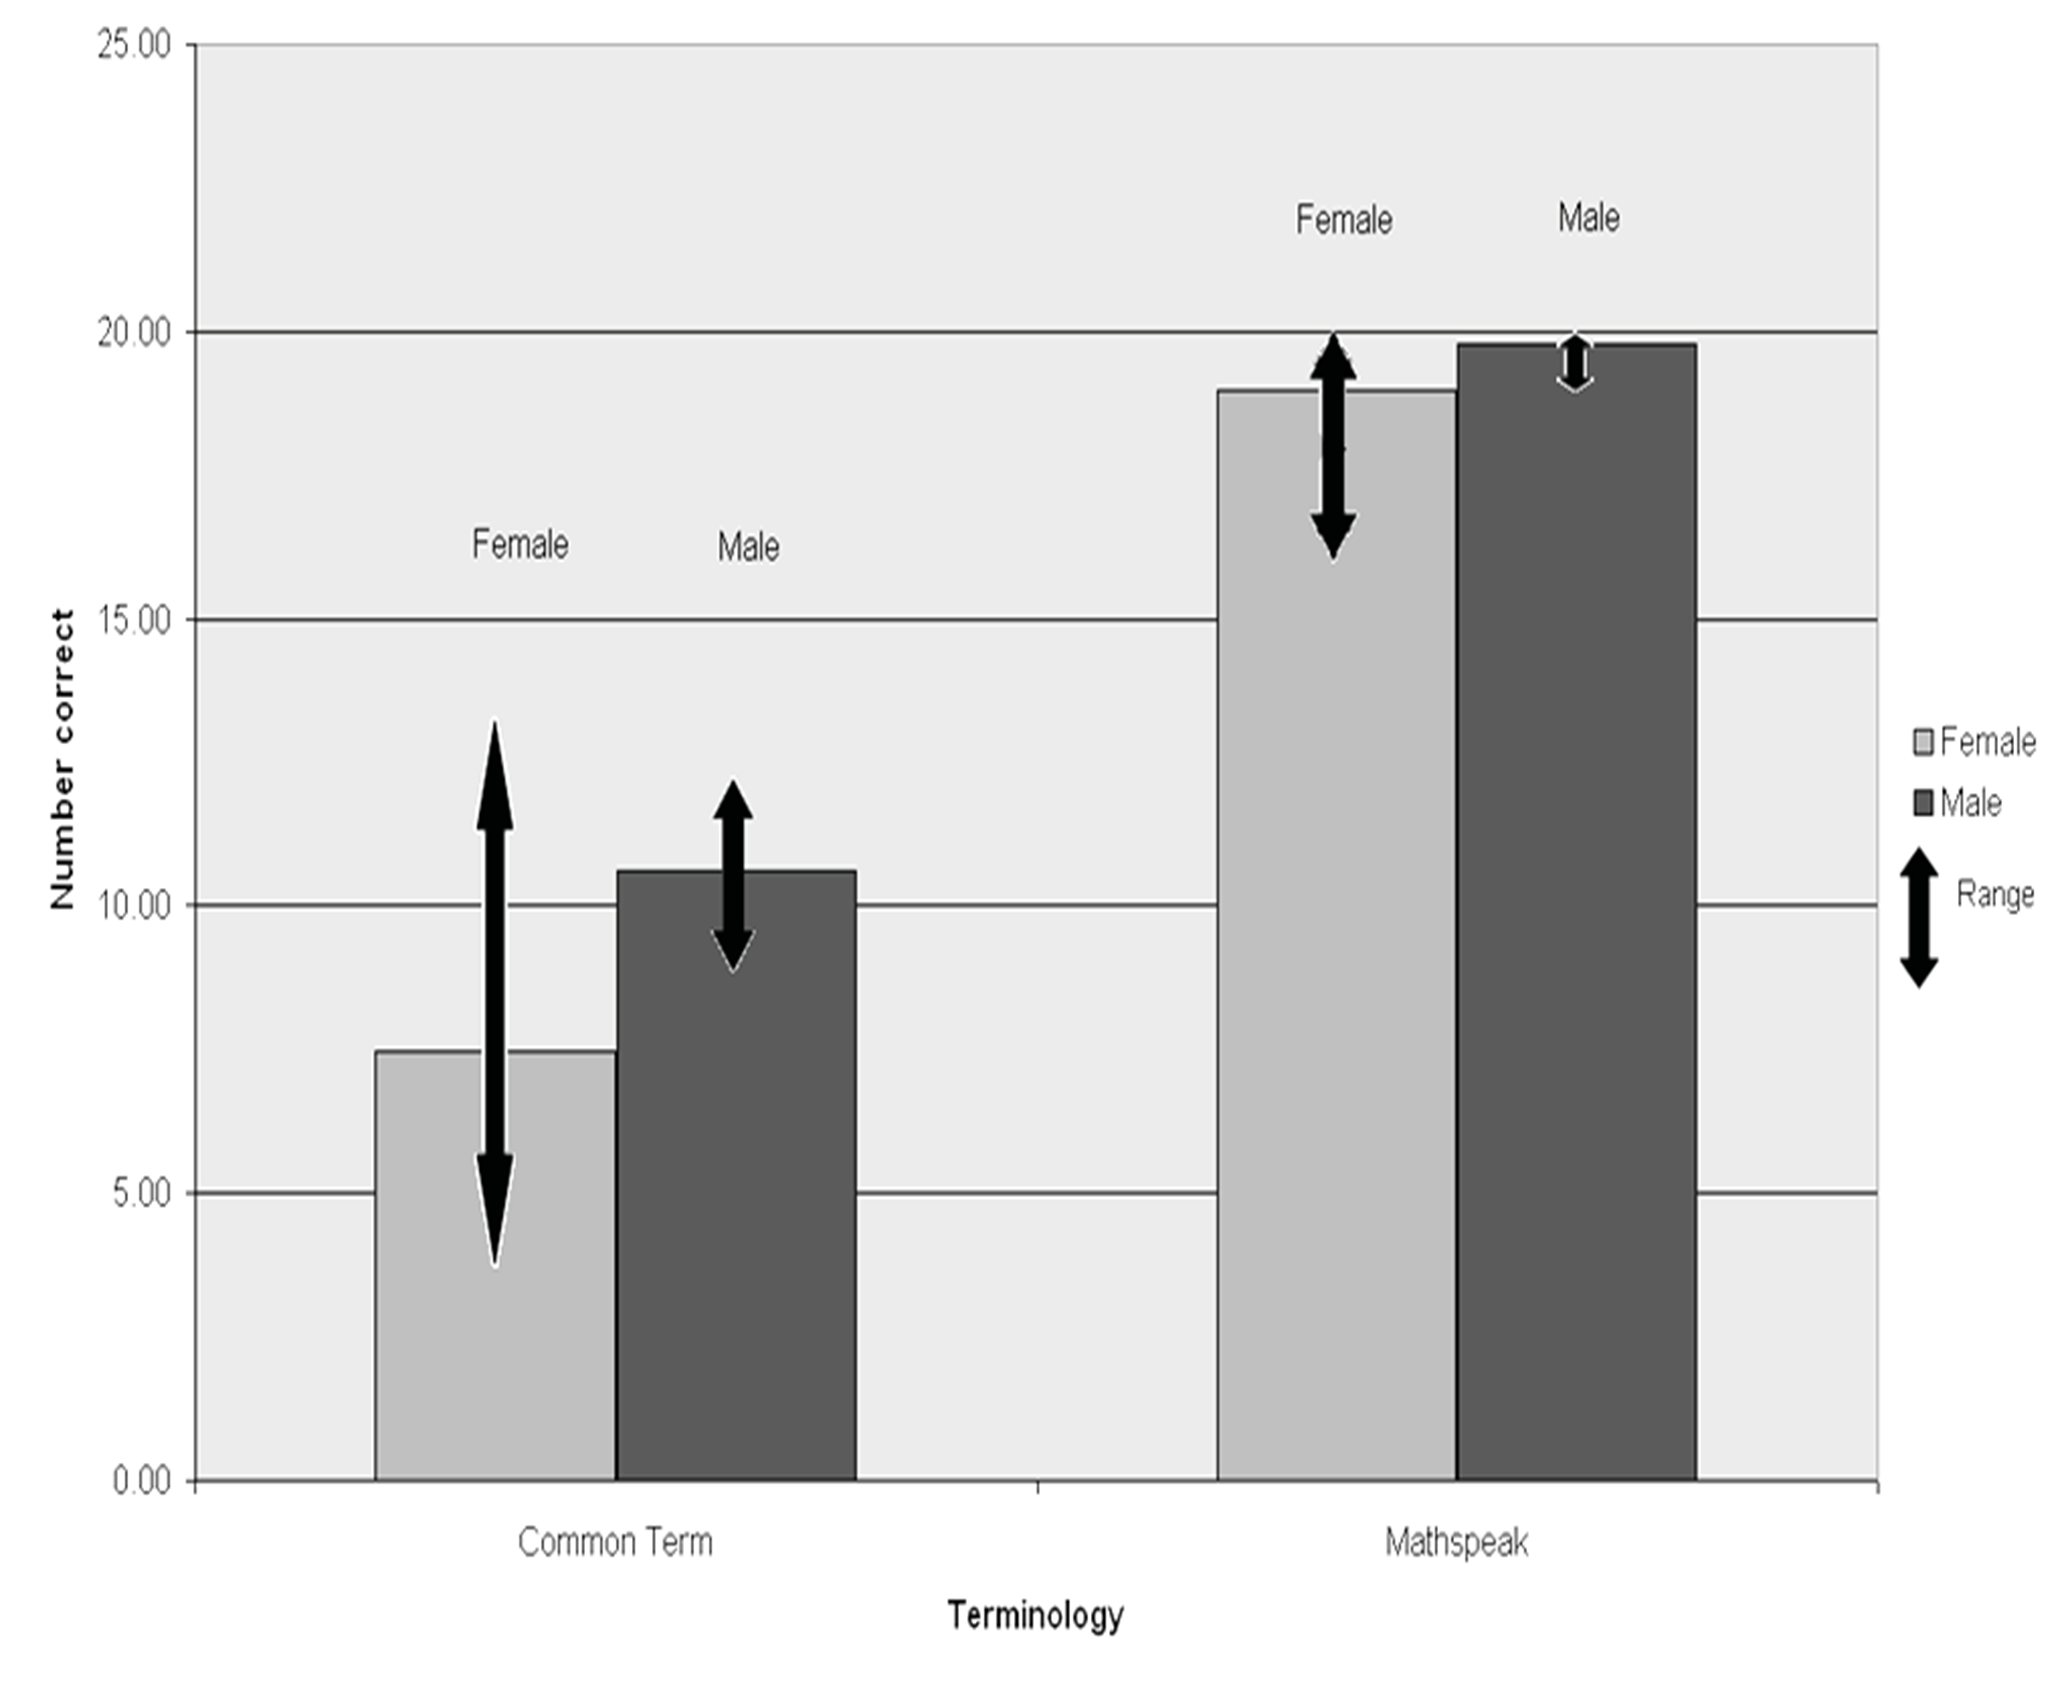
\includegraphics[width=1\textwidth]{images/fig1.png}
    \caption{Number of expressions correctly interpreted for the two types of terminology.}
    \label{Figure 1}
\end{figure*}

\section*{DISCUSSION}
The findings of the present study demonstrate that MathSpeak is efficacious for reducing ambiguity in spoken mathematics. Significantly more mathematical expressions were correctly interpreted when MathSpeak terminology was used compared to expressions rendered with common terminology. In fact, performance with MathSpeak was close to perfect. Without MathSpeak, performance did not differ from chance. Furthermore, MathSpeak rules appear to be easy to learn. The instructional phase during which MathSpeak rules were taught lasted for only four minutes and even with this short instructional time, performance was almost perfect.

Production of non-ambiguous auditory renderings of mathematics has received little research attention. A couple of publications address spoken mathematics, but they do not provide a systematic comprehensive system for disambiguation as with MathSpeak. These two publications, the Handbook of Spoken Mathematics: Larry’s Speakeasy (Lawrence Livemore National Disabilities Services, n.d.) and the National Braille Association Tape Recording Manual (National Library Service for the Blind and Physically Handicapped, n.d.) basically consist of non-rigorous informal guidelines for how humans should read equations aloud. A non-published doctoral thesis (Raman, 1994) on an Audio System for Technical Readings (ASTER) exists. The primary purpose of ASTER is to produce synthetic speech from literary texts and highly technical documents (LaTeX) code. The thesis does make a few suggestions for disambiguation, however, it is not the primary purpose of the thesis and the suggestions are minor and isolated to only a few instances of possible ambiguity. A comprehensive set of rules for disambiguation is not addressed nor provided by Raman’s thesis. In addition to the above, conference presentations and symposiums concerning conversion of printed mathematics into audio renderings and increasing the accessibility of STEM materials for the blind and visually impaired have been held (Annamalai, Gopal, Gupta, Karshmer, \& Guo, 2003; Batusic, Meisenberger, \& Stoger, 1996; Duke, 2004; Gardner, 2002; Gardner, Steward, Francioni, \& Smith, 2002; Miensenberger, Batusic, \& Stoger, 1998; Suzuki, Tamari, Fukuda, Uchida, \& Kanahori, 2003; Thompson, 2005). These presentations and symposiums have not produced a comprehensive set of rules for disambiguation. MathSpeak appears to be the only comprehensive set of rules for reducing multiple interpretations that arise from spoken mathematics.

The present study could not address all possible instances of potential ambiguity addressed by MathSpeak. The rules for those non-addressed instances were developed through the same process as those tested for efficacy. Therefore, it is likely that the non-tested MathSpeak rules would demonstrate similar degrees of efficacy.

The gender effect was unexpected. An artifact arising from the much smaller number of males relative to females and the relatively small number of males overall is a likely cause of the gender difference. Participants were solicited from an undergraduate education course and the relative abundance of females compared to males is typical of education classes. Regardless of this unexpected result, non-overlapping distributions for expression spoken with MathSpeak and those spoken with common everyday terminology firmly establishes MathSpeak efficacy for disambiguation of spoken mathematics.

Although the present study clearly establishes the efficacy of MathSpeak for enhancing spoken communication of mathematics, it should be remembered that ambiguous communication of mathematics is only one barrier inhibiting access to STEM based knowledge, education, and careers. Widespread implementation of MathSpeak will help to remove this specific barrier for individual who have print disabilities and may facilitate communication across professionals in STEM fields. Removing this communication barrier, however, is not sufficient. Development of additional technologies and elimination of arcane beliefs about careers in STEM by people who have blindness, low vision, or other print disabilities are also necessary.

\section*{ACKNOWLEDGEMENTS}
The authors wish to thank Jonathan Williford, Eric Graves, Sam Matthew, and the Purdue AAC research group for their help in this research project.

\section*{AUTHOR INFO}
\textbf{Mick Isaacson}\\
Department of Educational Studies\\ 
Purdue University\\
\href{mailto:isaacsom@purdue.edu}{isaacsom@purdue.edu}\\

\textbf{Dave Schleppenbach}\\
gh LLC\\
Purdue Research Park\\

\textbf{Lyle L. Lloyd}\\
Department of Speech, Language, and Hearing Sciences\\
Purdue University\\

\end{large}
\clearpage
\section*{REFERENCES}\par 

\leftskip 0.25in
\parindent -0.25in 
%%%
Americans with Disabilities Act (ADAOHIO). (2002). \textit{Census data on people with disabilities: interesting facts}. Retrieved November 16, 2009 from \url{http://www.ilru.org/healthwellness/html/census.html}

Annamalai, N., Gopal, D., Gupta, G., Karshmer, A., \& Guo, H. (2003). INSIGHT: A comprehensive system for translating Braille based mathematical documents into LaTex. \textit{Proceedings of the International Conference on Human Computer Interaction}, 1245-1249.

Batusic, M., Meisenberger, K., \& Stoger, B. (1996). Access to mathematics for the blind – Defining HrTeX standard.\textit{Proceedings of the 5th International Conference on Computers helping People with Special Needs}, 609-616.

Burstahler, S. (1994). \textit{Increasing the representation of people with disabilities in science, engineering, and mathematics}. Retrieved November 16, 2009, from \url{http://www.washington.edu/doit/Brochures/Careers/representation.html}

Committee on Equal Opportunities in Science and Engineering (CEOSE). (2007). \textit{CEOSE Mini-Symposium on Institutions Serving Persons with Disabilities in STEM Report}. Retrieved June 24, 2009, from \url{http://www.nsf.gov/od/oia/activities/ceose/ reports/ CEOSE-Mini-symposium-Report-Final.pdf- 2008-03-22}

Duke, W. (2004). A new math language for blind students. \textit{Proceedings of the CSUN International Conference on Technology and Persons with Disabilities, session 65}.

Gardner, J. A. (2002). Access by blind students and professionals to mainstream math and science. In K. Meisenberger, J. Klaus, \& W. Zagler (Ed.), \textit{Proceedings of the 8th International Conference on Computers Helping People with Disabilities, 2398}, 502-507.

Gardner, J. A., Steward, R., Francioni, J., \& Smith, A. (2002). Tiger, AGC, and WinTriangle, removing the barrier to SEM education. \textit{Proceedings of the CSUN International Conference on Technology and Persons with Disabilities, session 299}.

Lawrence Livermore National Disabilities Services. (n.d.). \textit{Handbook of Spoken Mathematics: Larry’s speak}. Livermore, CA.

Miensenberger, K., Batusic, M., \& Stoger, B. (1998). LABRA\-DOOR: LaTex to Braille door. \textit{Proceedings of the Conference on Telematics in the Education of the Visually Handicapped, Paris, France}. Retrieved April 5 from \url{http://www.snv.jussieu.fr/inova/publi/ntevh/labradoor.htm}

Raman, T.V. (1994). Audio System for Technical Readings. \textit{Unpublished doctoral dissertation}, Cornell University, Ithica, New York.

Suzuki, M., Tamari, F., Fukuda, R., Uchida, S. \& Kanahori, T. (2003). An integrated OCR system for mathematical documents. \textit{Proceedings of ACM Symposium on Document Engineering}, 95-104.

Thompson, D.M. (2005). LaTex: Physics and mathematics for the blind or visually impaired. \textit{Proceedings of the CSUN International Conference on Technology and Persons with Disabilities, session 2552}.

U.S. Census Bureau (2003). \textit{American fact finder}. Retrieved Nov 16, 2009 from \url{http://factfinder.census.gov/home/staff/main .html?_lang=en}.

\end{document}
